%!TEX TS-program = xelatex
\documentclass[]{friggeri-cv}
\usepackage{afterpage}
\usepackage{hyperref}
\usepackage{color}
\usepackage{xcolor}
\hypersetup{
    pdftitle={},
    pdfauthor={},
    pdfsubject={},
    pdfkeywords={},
    colorlinks=false,       % no lik border color
   allbordercolors=white    % white border color for all
}
\addbibresource{bibliography.bib}
\RequirePackage{xcolor}
\definecolor{pblue}{HTML}{0395DE}

\usepackage{enumitem}

\begin{document}
\header{Victor M.}{Mendiola-Lau}{Computer Scientist, Researcher and Software Engineer}
      
% Fake text to add separator      
\fcolorbox{white}{gray}{\parbox{\dimexpr\textwidth-2\fboxsep-2\fboxrule}{%
.....
}}

% In the aside, each new line forces a line break
\begin{aside}
  \section{Address}
    Ayuntamiento 7375, 
    Havana, Cuba
    ~
    ~
    ~
  \section{Telephone}
    (+53)5 413 2909 (cell)
  	(+53)7 873 0125 (home)
    ~
    ~
    ~
  \section{Mail}
    \href{mailto:ryuzakyl@gmail.com}{\textbf{ryuzakyl@}gmail.com}
	~
	~    
    ~
  \section{Web profiles}
    \href{https://github.com/ryuzakyl}{{\scriptsize github.com/ryuzakyl}}
    \href{https://independent.academia.edu/VictorMendiolaLau}{{\scriptsize academia.edu/VictorMendiolaLau}}
    \href{https://www.linkedin.com/in/VictorMendiolaLau}{{\scriptsize linkedin.com/in/VictorMendiolaLau}}
	\href{https://www.researchgate.net/profile/Victor_Mendiola-Lau}{{\scriptsize researchgate.net/Victor\char`_Mendiola-Lau}}
    ~
    ~
    ~
  \section{Personal Skills}
    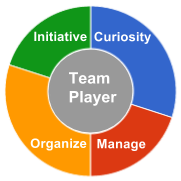
\includegraphics[scale=0.62]{img/personal.png}
    ~
%    ~
%  \section{Programming}
%    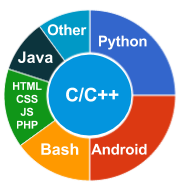
\includegraphics[scale=0.62]{img/programming.png}
%    ~
\end{aside}

\section{Academia}
\begin{entrylist}
  \entry
    {10/17 - Now}
    {Assistant Professor}
    {University of Havana, Cuba}
    {Math instructor of topics such as Set theory, Functions, Calculus, Numerical math and Ordinary Differential Equations.\\}
  
  \entry
    {09/13 - 09/17}
    {Researcher}
    {CENATAV, Havana, Cuba}
    {Design and development Pattern Recognition Systems. Junior researcher and PhD. student. Interest on topics like Computer Vision, Data Analysis, Data Representation, Clustering and Classification. Technologies: Python, Numpy, SciPy, Matplotlib, scikit-learn, etc.\\}
    
  \entry
    {06/12 - 07/12}
    {Research internship}
    {CENATAV, Havana, Cuba}
    {Design and implementation of an iris encoding method based on Functional Data Analysis (FDA).\\}
    
  \entry
    {09/10 - 06/13}
    {Assistant Instructor}
    {University of Havana, Cuba}
    {Instructor of Programming and Algorithms for Mathematics students in the Faculty of Mathematics and Computer Science (MATCOM).\\}
\end{entrylist}

\section{Software Engineering}
\begin{entrylist}
  \entry
    {09/17 - Now}
    {Full Stack Web Developer}
    {HRSG - Human Resource Systems Group Ltd.}
    {Web-based applications as solutions to workforce management. Technologies: PHP, HTML, CSS3, JavaScript, jQuery, MySQL, etc.\\} 
  
  \entry
    {02/16 - 03/16}
    {Backend Ruby/Rails Developer}
    {Ksabes, Havana, Cuba}
    {Completely engineered and developed an API relying on Json Web Token (JWT) for authentication.\\}
  
  \entry
    {09/14 - 01/15}
    {Ruby Developer}
    {IRStrat, México D.F., México}
    {Completely engineered and developed a multi-threaded and concurrent service for consuming real time stock market data.\\}

  \entry
    {09/13 - 09/17}
    {Software Engineer}
    {CENATAV, Havana, Cuba}
    {Full Stack Desktop Developer using the .NET Framework, specifically with C\#. Efficient algorithm design and implementation in C/C++. Integration of .NET desktop applications with C/C++ libraries via PInvoke.\\}
\end{entrylist}

\pagebreak

\section{Education/Academic background}
\begin{entrylist}
%  \entry
%    {2009 - 2012}
%    {Master's Degree in Computer Engineering}
%    {Università di Pisa, Italy}
%    {Curriculum Networking and Multimedia.\\
%    Main subjects: Network Applications, Systems Architecture and Security, Mobile Applications, Multemedia Information            Processing.\\
%    \emph{Title of the Thesis: "A Handoff Algorithm based on Link Quality Prediction for Mass Transit Wireless Mesh Networks"      .}\\
%    \emph{Relators: Prof. Enzo Mingozzi, Ing. Carlo Vallati, Prof. Luciano Lenzini.}\\}

  \entry
    {2008 - 2013}
    {B.Sc. in Computer Science}
    {University of Havana, Cuba}
    {B.Sc. \textbf{\emph{summa cum laude}} in Computer Science. Main subjects: Programming, Algorithms and Data Structures, Computational Complexity Theory, Matematics, Operational Research, Numerical Matematics and Artificial Intelligence.\\
    \emph{Title of the Thesis: "Iris Recognition using Functional Data Analysis (FDA)".}}

%  \entry
%    {2004 - 2007}
%    {Bachelor Diploma}
%    {IPVCE Vladimir Ilich Lenin, Havana, Cuba}
%    {Bachelor diploma with focus on these subjects: Matematics and Computer Science.}
\end{entrylist}

\section{Languages}
\begin{entrylist}
  \entry
    {\textbf{Spanish}}
    {}
    {}
    {Native tongue}      

  \entry
    {\textbf{English}}
    {}
    {}
    {Graduated \textbf{\emph{summa cum laude}} at \emph{Abraham Lincoln} Languages School.}

  \entry
    {\textbf{French}}
    {}
    {}
    {Diplôme d'études en langue française (\textbf{DELF B1}) à l'Alliance française.}
\end{entrylist}

\section{Certifications \& Training courses}
\begin{entrylist}
  \entry
    {2014}
    {(Postgraduate) Methodologies of Scientific Research}
    {CENATAV, IDICT}
    {\emph{Demistify research and research methods. Outline of the fundamentals of doing research.}}
\end{entrylist}

\begin{entrylist}    
  \entry
    {2013}
    {(Tutorial) Fundamentals of Iris Recognition}
    {CIARP 2013 Congress}
    {\emph{Tutorial presented by Professor Tieniu Tan on the roadmap of Iris Recognition.}}

  \entry
    {}
    {(Tutorial) Big Data Analytics}
    {CIARP 2013 Congress}
    {\emph{Mining Uncertain and Probabilistic Data for Big Data Analytics by Professor Jian Pei.}}
    
  \entry
    {}
    {(Undergraduate) \LaTeX}
    {University of Havana}
    {\emph{Introduction to the document description language built on top of \TeX.}}
\end{entrylist}
       
\begin{entrylist}
  \entry
    {2012}
    {(Postgraduate) Advanced Data Structures}
    {University of Havana}
    {\emph{Introduction concepts such as Amortized Analysis, Fibonacci Heaps, Splay Trees, etc.}}      

  \entry
    {}
    {(Undergraduate) Business Intelligence}
    {University of Havana}
    {\emph{Introduction to the core concepts of modern Business Intelligence processes.}}

  \entry
    {}
    {(Undergraduate) Introduction to Cryptography}
    {University of Havana}
    {\emph{Introduction to the fundamentals of modern Cryptography.}}
\end{entrylist}

\begin{entrylist}
  \entry
    {2011}
    {(Undergraduate) Introduction to Computer Vision}
    {University of Havana}
    {\emph{Foundations of Computer Vision with OpenCV.}}      

  \entry
    {}
    {(Undergraduate) Introduction to Computer Graphics}
    {University of Havana}
    {\emph{Foundations of Computer Graphics.}}
\end{entrylist}

\pagebreak

\section{Publications}
\begin{paperlist}
  \paperentry
    {2017}
    {}
    {}
    {
		\emph{(Accepted)} \textbf{Victor Mendiola-Lau}, Francisco J. Silva Mata, Yenisel Plasencia Calaña, Isneri Talavera Bustamante and Maria De Marsico. ``Bio-chemical Data Classification by Dissimilarity Representation and Template Selection." \emph{CIARP}, 2017.
    }
\end{paperlist}

\vspace{0.5cm}

\begin{paperlist}
  \paperentry
    {2016}
    {}
    {}
    {
		\textbf{Victor Mendiola-Lau}, F.J. Silva-Mata, Y. Martínez-Díaz, I. Talavera Bustamante and M. De Marsico. ``Exploratory Data Analysis Combined with Entropy-based Template Selection for the Identification of Mixed Substances."	 \emph{CAC}, 2016.
    }
\end{paperlist}

\begin{paperlist}
  \paperentry
    {}
    {}
    {}
    {
		\textbf{Victor Mendiola-Lau}, Francisco J. Silva Mata, Yoanna Martínez-Díaz, Isneri Talavera Bustamante, Maria De Marsico. ``Hierarchical Clustering Combined with Entropy Based-template Selection and SVM Classification for the Identification of Mixed Substances by Means of UV and GC Analytical Technique." \emph{Informática}, 2016.
    }
\end{paperlist}

\begin{paperlist}
  \paperentry
    {}
    {}
    {}
    {
		\textbf{Victor Mendiola-Lau}, Francisco J. Silva Mata, Yoanna Martínez-Díaz, Isneri Talavera Bustamante and Maria De Marsico. ``Automatic classification of herbal substances enhanced with an entropy criterion." \emph{CIARP}, 2016.
    }
\end{paperlist}

\vspace{0.5cm}

\begin{paperlist}
  \paperentry
    {2015}
    {}
    {}
    {
		Francisco J. Silva-Mata, \textbf{Victor Mendiola-Lau}, Isneri Talavera-Bustamante and Yoanna Martínez-Díaz. ``Automatic processing of TLC images for discovering clusters and performing classification tasks of herbal substances. Case of study". \emph{SSC14}, 2015.
    }
\end{paperlist}

\begin{paperlist}
  \paperentry
    {}
    {}
    {}
    {
		Francisco J. Silva Mata, Dania P.- Muñoz, Stefano Berretti, \textbf{Victor Mendiola-Lau}, Isneri Talavera Bustamante, Noslen Hernández, Yoanna Martínez-Díaz, Angel Augier . ``Alineación de señales e imágenes durante la aplicación del análisis de datos funcionales: Ejemplos prácticos en señales e imágenes quimiométricas y biométricas." \emph{RCF}, 2015.
    }
\end{paperlist}

\begin{paperlist}
  \paperentry
    {}
    {}
    {}
    {
		Francisco J. Silva Mata, Dania P.- Muñoz, \textbf{Victor Mendiola-Lau}, Isneri Talavera Bustamante, Angel Augier. ``Criterios y métodos de selección de bases y su impacto en el análisis de datos funcionales: Algunos ejemplos en biometría". \emph{RCF}, 2015.
    }
\end{paperlist}

\begin{paperlist}
  \paperentry
    {}
    {}
    {}
    {
		\textbf{Victor Mendiola-Lau}, Isneri Talavera Bustamante and Maria de Marsico. ``Clustering of simple and multi-way spectral data on the dissimilarity representation." \emph{Serie Azul CENATAV}, 2015.
    }
\end{paperlist}

\begin{paperlist}
  \paperentry
    {}
    {}
    {}
    {
		Francisco J. Silva Mata,  Isneri Talavera, \textbf{Victor Mendiola-Lau}, Yoanna Martínez Díaz, Anier Revilla Eng. ``Clasificación de Sustancias Vegetales con el uso de un Sistema Automatizado para el proceso de Imágenes de TLC". En: IX Congreso de Ciencias, Tecnología e Innovación Química, Quimicuba 2015, La Habana, Cuba, 13-16 de octubre de 2015.
    }
\end{paperlist}

\begin{paperlist}
  \paperentry
    {}
    {}
    {}
    {
		Dania Porro, Isneri Talavera, Robert Duin, Gabriela Barcas, \textbf{Victor Mendiola-Lau}. ``Comparación De Diferentes Formas De Representación De Datos Espectrales Para Clasificación De Sustancias." En: IX Congreso de Ciencias, Tecnología e Innovación Química, Quimicuba 2015, La Habana, Cuba, 13-16 de octubre de 2015.
    }
\end{paperlist}

\begin{paperlist}
  \paperentry
    {}
    {}
    {}
    {
		Francisco J. Silva Mata, \textbf{Victor Mendiola-Lau}, Anier Revilla, Isneri Talavera, Angel Augier, Stefano Berretti y Yoanna Martínez. Optimización de los Modelos Funcionales para Objetos Biométricos. \emph{RECPAT}, 2015.
    }
\end{paperlist}

\vspace{0.5cm}

\begin{paperlist}
  \paperentry
    {2014}
    {}
    {}
    {
		Francisco J. Silva-Mata, Dania P.-Muñoz, \textbf{Victor Mendiola-Lau}, Isneri Talavera-Bustamante, Angel Augier. ``Criteria and methods of selection of bases and their impact in functional data analysis. Some examples in biometrics". \emph{CIOFF}, 2014.
    }
\end{paperlist}

\begin{paperlist}
  \paperentry
    {}
    {}
    {}
    {
		Francisco J. Silva-Mata, Dania P.-Muñoz, Stefano Berretti, \textbf{Victor Mendiola-Lau}, Isneri Talavera-Bustamante, Noslen Hernández, Yoanna Martínez-Díaz, Angel Augier. ``Signal and image alignment during the application of functional data analysis. Practical examples of chemometrics and biometrics". \emph{CIOFF}, 2014.
    }
\end{paperlist}

\begin{paperlist}
  \paperentry
    {}
    {}
    {}
    {
		\textbf{Victor Mendiola-Lau}, Francisco J. Silva-Mata, Dania P.-Muñoz, Isneri Talavera-Bustamante. ``APIris: Nueva Plataforma Automatizada para el Reconocimiento de Iris". \emph{RECPAT}, 2014.
    }
\end{paperlist}

\begin{paperlist}
  \paperentry
    {}
    {}
    {}
    {
		Francisco J. Silva-Mata, Dania P.-Muñoz, \textbf{Victor Mendiola-Lau}, Anier Revilla-Eng, Isneri Talavera-Bustamante. ``Criterios y métodos para representar imágenes biométricas usando FDA". \emph{RECPAT}, 2014.
    }
\end{paperlist}

\vspace{0.5cm}

\begin{paperlist}
  \paperentry
    {2013}
    {}
    {}
    {
		Dania P.-Muñoz, Francisco J. Silva-Mata, \textbf{Victor Mendiola-Lau}, Noslen Hernández, and Isneri Talavera-Bustamante. ``A new iris recognition approach based on a functional representation". \emph{CIARP}, 2013.
    }
\end{paperlist}

\vspace{0.5cm}

\begin{paperlist}
  \paperentry
    {2011}
    {}
    {}
    {
		Javier Guillot-Jiménez, \textbf{Victor Mendiola-Lau}, Benny Jon-Robaina, Daniel A. Mesejo-León, Omar Salas-García and Haydée Guillot-Jiménez. ``SIMPLER: SIMPLER: desde el MERX hasta las Bases de Datos". \emph{COMPUMAT}, 2011.
    }
\end{paperlist}
\\
\section{Technologies}
\begin{entrylist}
  \entry
    {\textbf{Languages}}
    {}
    {}
    {\textbf{C\#} (+8 years), \textbf{Python} (+6 years), \textbf{C/C++} (+4 years), \textbf{Ruby} (+3 years). Other languages include \textbf{Java}, \textbf{PHP} and \textbf{Go}. }

  \entry
    {\textbf{IDEs}}
    {}
    {}
    {\textbf{Visual Studio} (+8 years), \textbf{PyCharm} (+5 years), \textbf{RubyMine} (+3 years). Other IDEs and Text Editors include \textbf{PhpStorm}, \textbf{Clion}, \textbf{VS Code} and \textbf{Sublime Text}.}

  \entry
    {\textbf{DVCS}}
    {}
    {}
    {\textbf{Git} (+4 years) (GitHub, GitLab and Bitbucket).}
    
  \entry
    {\textbf{DBMS}}
    {}
    {}
    {\textbf{Microsoft SQL Server}, \textbf{PostgreSQL}, \textbf{MySQL} and \textbf{SQLite}.}

  \entry
    {\textbf{ML}}
    {}
    {}
    {The Python stack for Machine Learning and Scientific Computation: \textbf{Numpy}, \textbf{SciPy}, \textbf{Pandas}, \textbf{scikit-learn} and \textbf{Matplotlib}. Also the \textbf{MATLAB} Programming Language and environment.}
    
  \entry
    {\textbf{CV}}
    {}
    {}
    {\textbf{OpenCV}, \textbf{EmguCV} and \textbf{OpenCV-Python bindings}.}    
    
  \entry
    {\textbf{Web}}
    {}
    {}
    {\textbf{HTML}, \textbf{CSS3}, \textbf{JavaScript}, \textbf{jQuery}, etc. Some web frameworks like \textbf{Ruby on Rails} and \textbf{Django}.}    
    
  \entry
    {\textbf{OS}}
    {}
    {}
    {\textbf{Microsoft Windows} (XP, 7, 8, 8.1, 10) and \textbf{GNU/Linux} (Ubuntu, Linux Mint).}
\end{entrylist}
\\
\section{Other Accomplishments}
\begin{itemize}[noitemsep, nolistsep]

	\item Achieved a GPA of 5.13 over a scale of 5\footnote{The extra points were the result of outstanding academic achievements.}.\\

	\item ACM-ICPC Cuban Finals contestant (2011 and 2013 editions).\\

	\item Winner of the $1^{st}$ prize at the 2010-2011 Scientific Journal of the Faculty of Mathematics and Computer Science.\\
	
	\item I have made some contributions to the Wikipedia article entitled ``\emph{Computational complexity theory}".\\
		
	\item Winner of the silver medal in Mathematics of the $12^{ve}$ grade in La Habana.\\
	
	% \item From 2004 until 2007 was selected as part of advanced groups in Mathematics.\\	
	
	% \item Best candidate\footnote{Highest grade.} of the \emph{Plaza de la Revolución} locality at the IPVCE Vladimir Ilich Lenin admission tests in 2003-2004.\\	
	
	% \item Valedictorian from my elementary school in 2001.\\	
	
\end{itemize}

\end{document}
